%!TEX root = ./main.tex

\section{XG History}

\begin{frame}{Mobile has made a leap every 10 years}
  \centering
  \begin{tikzpicture}[
      gen/.style={draw=blue!55, fill=blue!6, rounded corners=3pt, minimum width=1.55cm, minimum height=0.78cm, align=center, font=\bfseries},
      note/.style={align=center, font=\scriptsize, text width=1.65cm},
      >=Latex
    ]
    \node[gen] (g1) at (0,0) {1G};
    \node[gen] (g2) at (2.15,0) {2G};
    \node[gen] (g3) at (4.3,0) {3G};
    \node[gen] (g4) at (6.45,0) {4G};
    \node[gen] (g5) at (8.6,0) {5G};
    \foreach \a/\b in {g1/g2,g2/g3,g3/g4,g4/g5}
      \draw[->, thick, blue!60] (\a) -- (\b);
    \node[note] at (0,-1.0) {Voice};
    \node[note] at (2.15,-1.0) {Text};
    \node[note] at (4.3,-1.0) {Web};
    \node[note] at (6.45,-1.0) {Video};
    \node[note] at (8.6,-1.0) {Connected\\things};
  \end{tikzpicture}

  \vspace{1.0em}
  \begin{tabular}{@{}lllll@{}}
    1980s & 1990s & 2000s & 2010s & 2020s \\
  \end{tabular}

  \vspace{0.8em}
  \small
  Each generation changed what people expected a phone to do.
  The device, radio link, and battery budget moved together.
\end{frame}

\begin{frame}{Every Generation Has Its Own Sound}
  \Large
  \blink{https://www.youtube.com/watch?v=0F8AmuobbZk}{Play the Nokia ringtone memory}.

  {\tiny
  Every time I hear this tune, I remember my youth, the beautiful days, and the people who made those days bright.}

  \vspace{0.8em}
  \normalsize
  \begin{itemize}
    \item A familiar sound carried a decade of mobile culture.
    \item Ringtones made the phone personal.
    \item Polyphonic audio showed that phones had become small media devices. 
    \begin{itemize}
      \item What makes a computer powerful?
      \item Compute throughput, memory capacity, memory bandwidth, storage capacity and speed, I/O bandwidth, processing latency, energy efficiency...
    \end{itemize}
  \end{itemize}

  
\end{frame}

% \begin{frame}{Applications follow capability}
%   \begin{columns}[T]
%     \column{0.46\textwidth}
%       \Large \textbf{The phone got stronger.}
%       \vspace{0.7em}

%       \normalsize
%       \begin{itemize}
%         \item More radio throughput
%         \item More local processing
%         \item Better screens, sensors, and storage
%         \item More energy demand
%       \end{itemize}

%     \column{0.54\textwidth}
%       \Large \textbf{The default app changed.}
%       \vspace{0.7em}

%       \normalsize
%       \begin{itemize}
%         \item 1G: voice on analog cellular links
%         \item 2G: text, contact lists, and ringtones
%         \item 3G: web, email, and early video calls
%         \item 4G: maps, streaming, and short video
%         \item 5G: connected things, sensing, and edge AI
%       \end{itemize}
%   \end{columns}

%   \vspace{0.5em}
%   \small
%   A new ``G'' matters when phones, radios, and nearby computing support a new daily habit.
% \end{frame}

\begin{frame}{1G: Mobile Voice}

  \begin{columns}[T,onlytextwidth]

    \column{0.46\textwidth}
      \centering
      \begin{figure}
        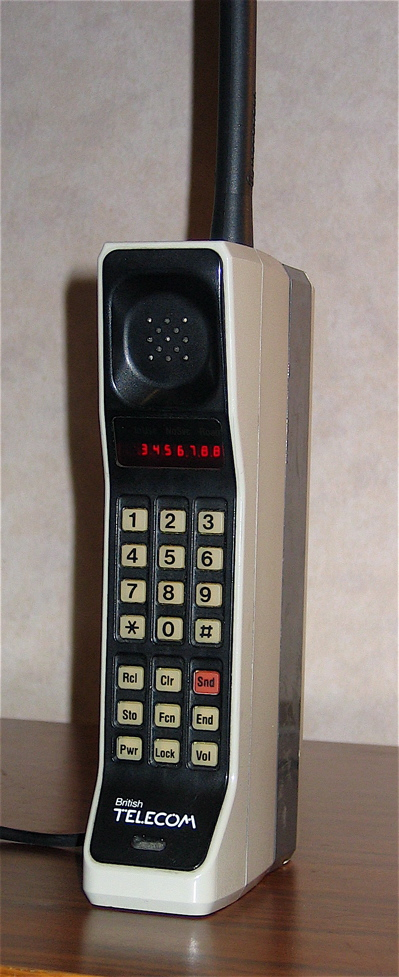
\includegraphics[height=0.64\textheight]
          {figure/xg/1g_dynatac.jpg}\\
        \vspace{0.3em}
        {\footnotesize The Motorola DynaTAC ``brick phone.''\par}
      \end{figure}

    \column{0.54\textwidth}

      \Large\textbf{The phone leaves the wall.}

      \vspace{0.8em}

      \normalsize
      \begin{itemize}
        \item Analog cellular voice
        \item Expensive devices and sparse coverage
        \item The core experience: calling from a car or the street
      \end{itemize}

  \end{columns}

\end{frame}

\begin{frame}{2G: Text goes mobile}
  \begin{columns}[T]
    \column{0.46\textwidth}
      \centering
      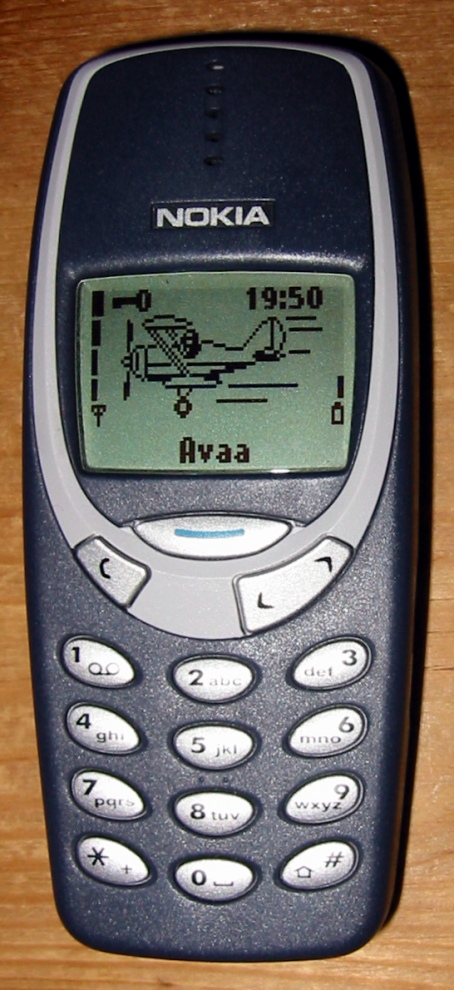
\includegraphics[height=0.64\textheight]{figure/xg/2g_nokia3310.jpg}\\
      \vspace{0.3em}
        {\footnotesize Nokia-style durable feature phones.\par}
    \column{0.54\textwidth}
      \Large \textbf{The phone becomes personal.}
      \vspace{0.8em}

      \normalsize
      \begin{itemize}
        \item Digital voice and SMS
        \item SIM cards, contacts, and prepaid plans
        \item Ringtones, Snake, and the always-on pocket device
      \end{itemize}

  \end{columns}
\end{frame}

\begin{frame}{3G: The web reaches the iPhone 4}
  \begin{columns}[T]
    \column{0.48\textwidth}
      \centering
      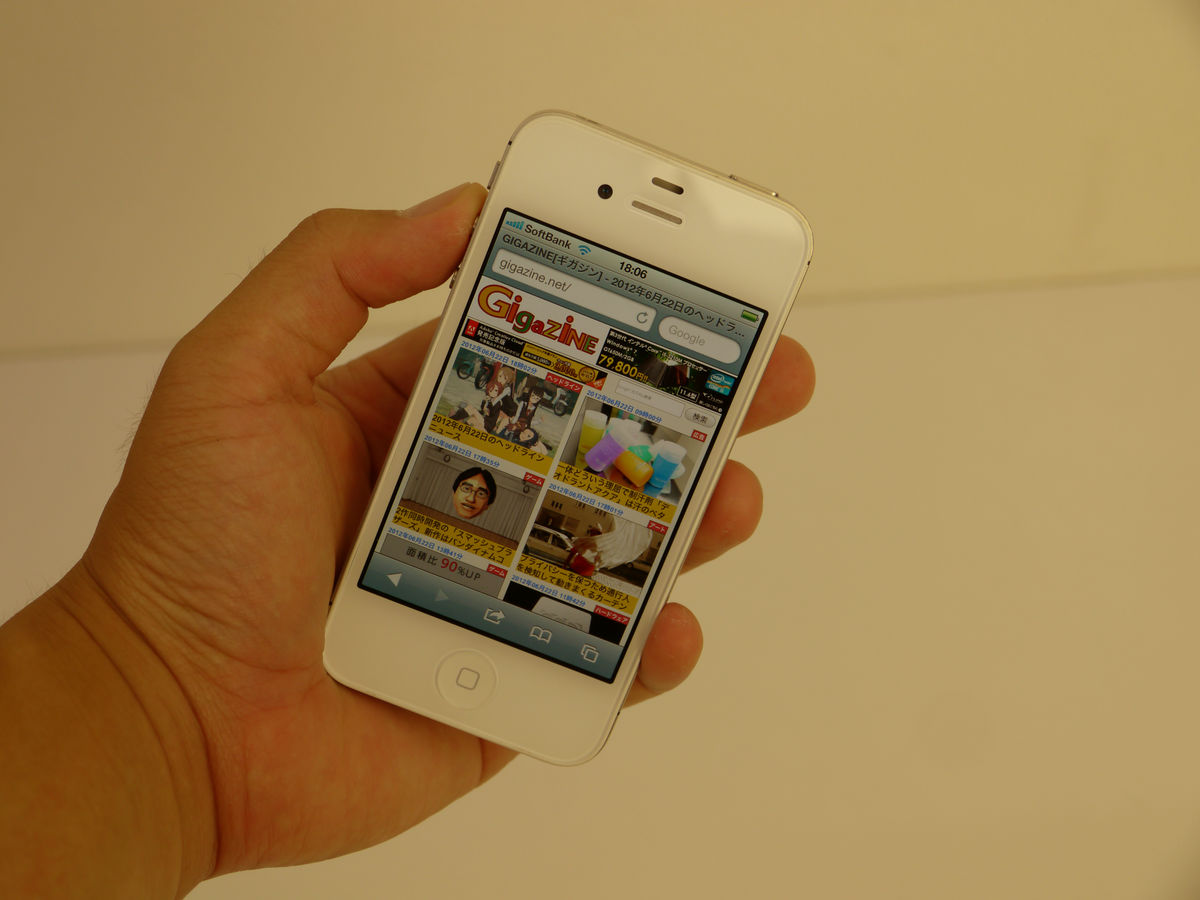
\includegraphics[width=\linewidth]{figure/xg/iphone4_white_web.jpg}\\
      \vspace{0.3em}
        {\footnotesize A white iPhone 4, a defining device of the 3G era, browsing the mobile web.\par}
    \column{0.52\textwidth}
      \Large \textbf{Data becomes the product.}
      \vspace{0.8em}

      \normalsize
      \begin{itemize}
        \item Mobile web, email, and app stores
        \item Camera phones and multimedia messages
        \item Early video calls over UMTS networks
      \end{itemize}


  \end{columns}
\end{frame}

\begin{frame}{4G: Video becomes normal}
  \begin{columns}[T]
    \column{0.50\textwidth}
      \centering
      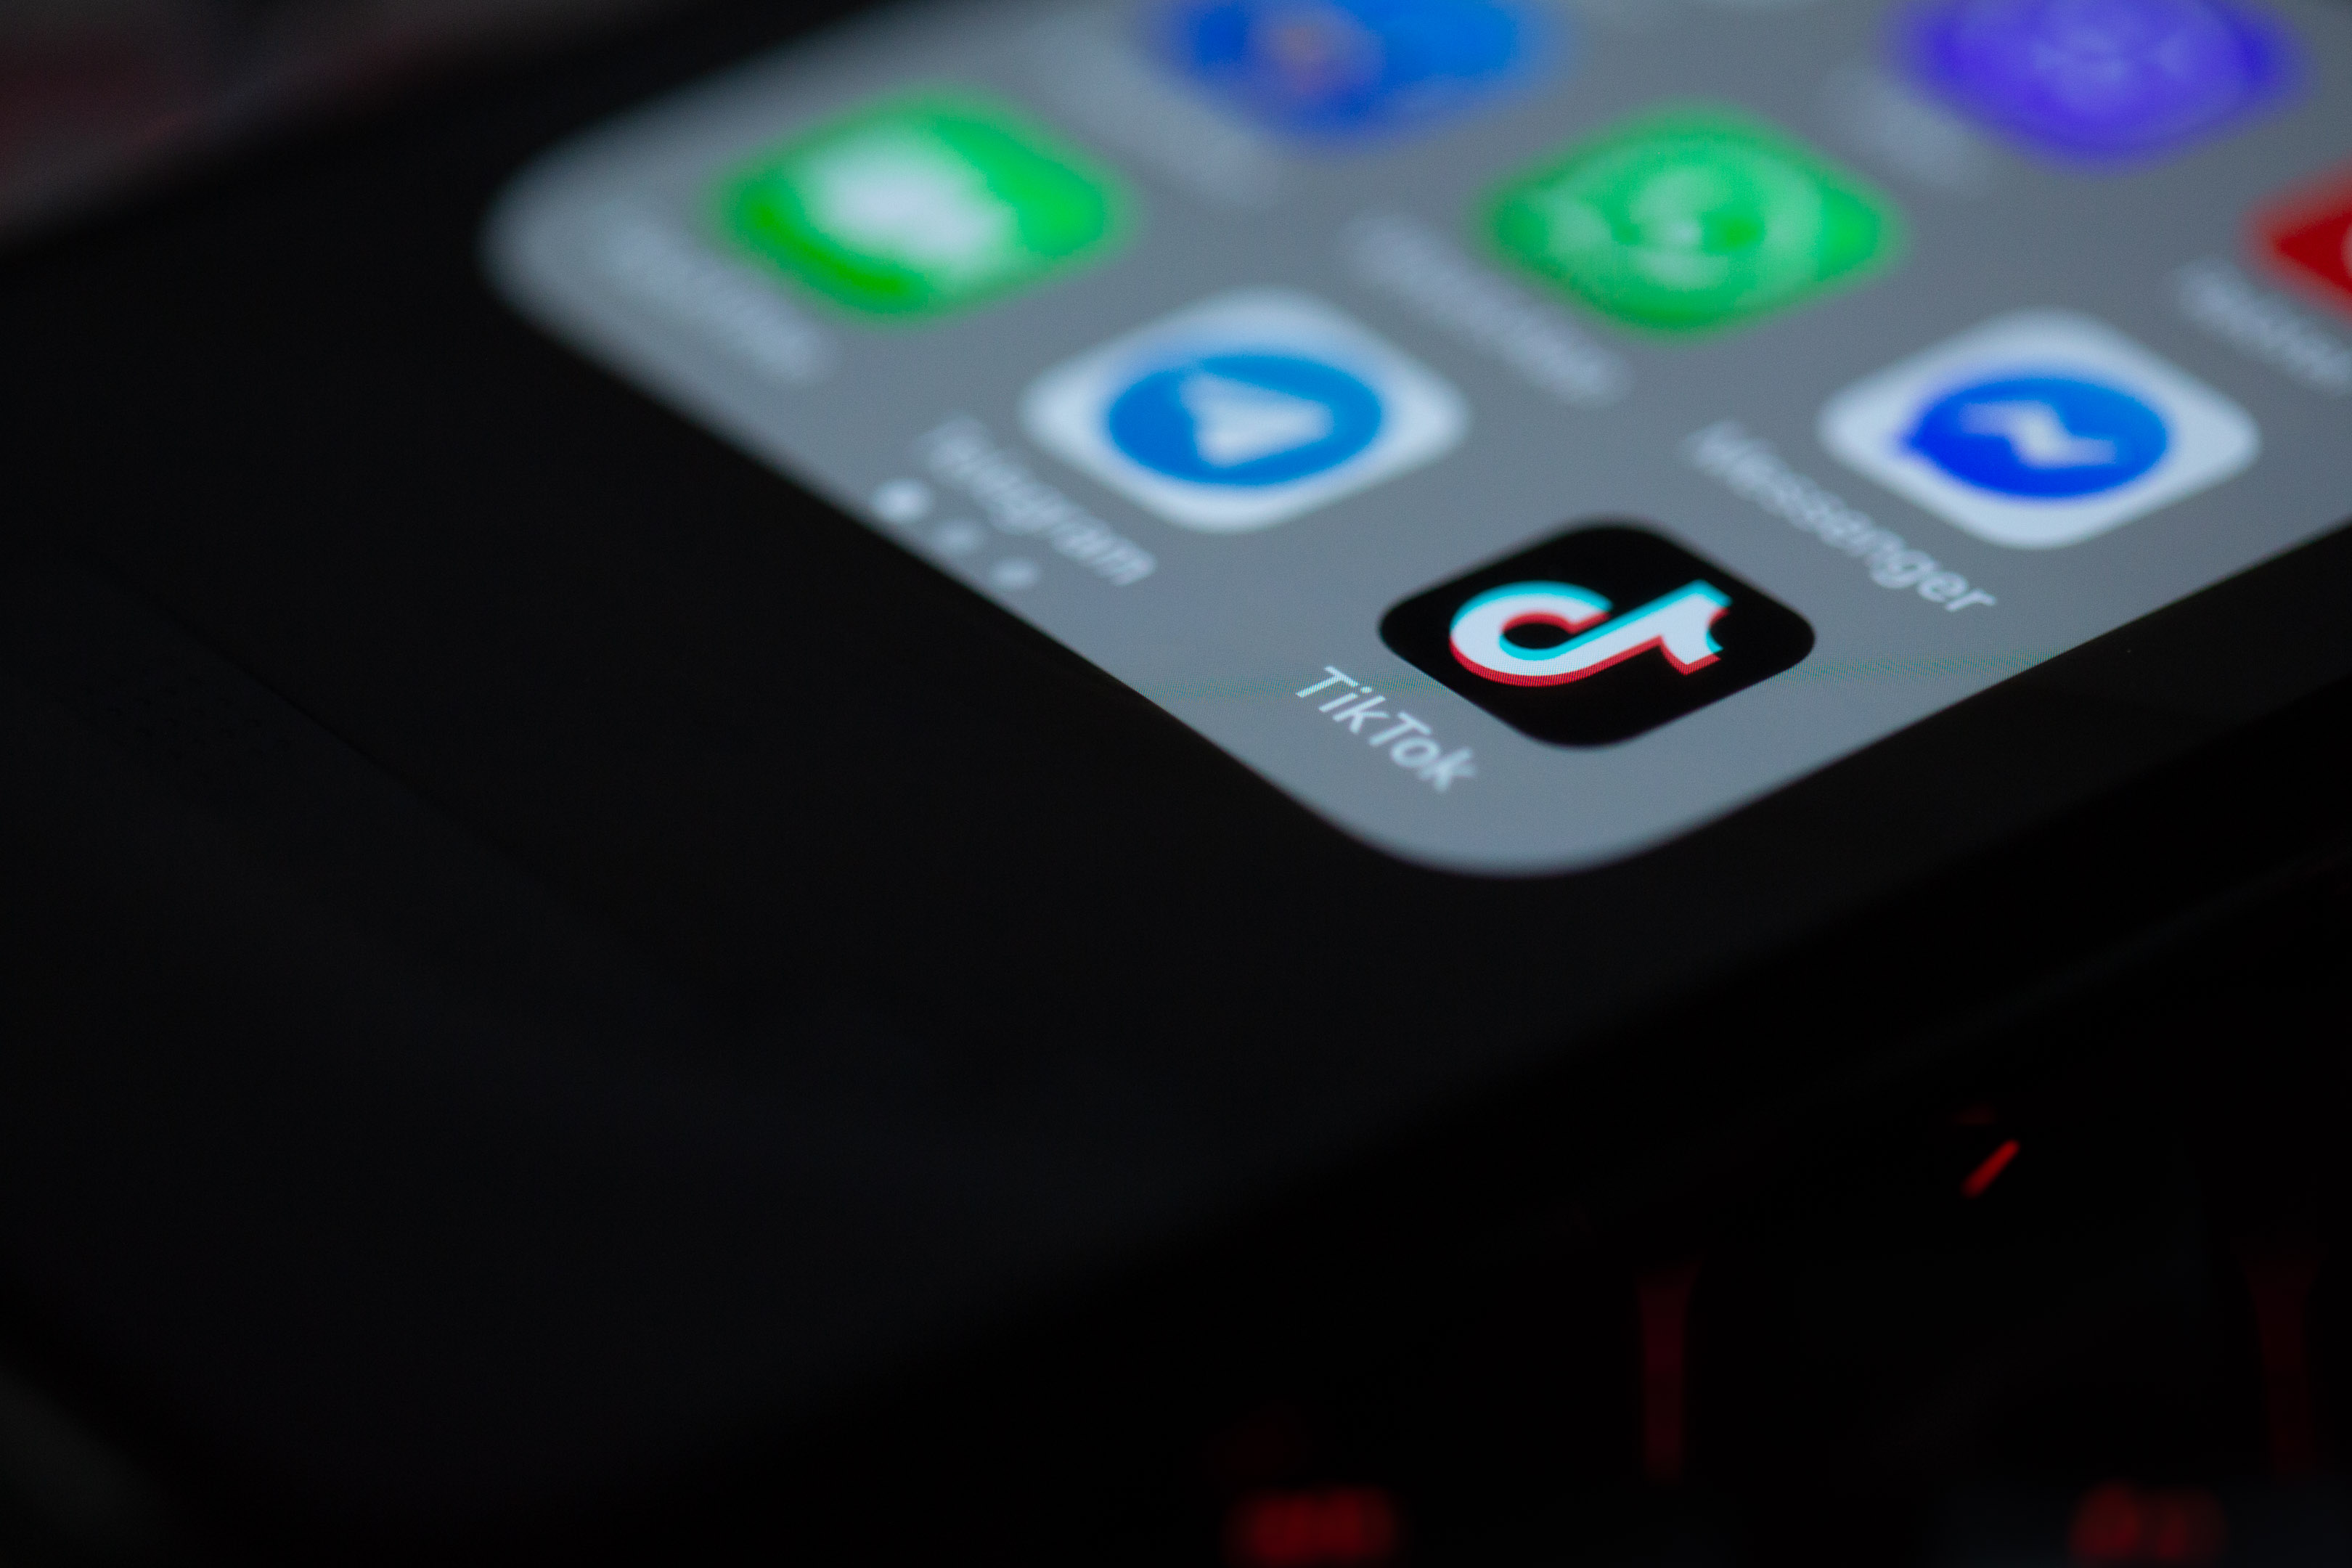
\includegraphics[width=\linewidth]{figure/xg/4g_tiktok_app.jpg}\\
      \vspace{0.3em}
        {\footnotesize TikTok and short-video apps.\par}
    \column{0.50\textwidth}
      \Large \textbf{The phone becomes a video network.}
      \vspace{0.8em}

      \normalsize
      \begin{itemize}
        \item LTE makes mobile broadband feel routine
        \item Streaming, ride sharing, maps, and live apps
        \item Short video turns uplink and downlink into daily traffic
      \end{itemize}

  \end{columns}
\end{frame}

\begin{frame}{5G: The network leaves the phone}
  \begin{columns}[T]
    \column{0.50\textwidth}
      \centering
      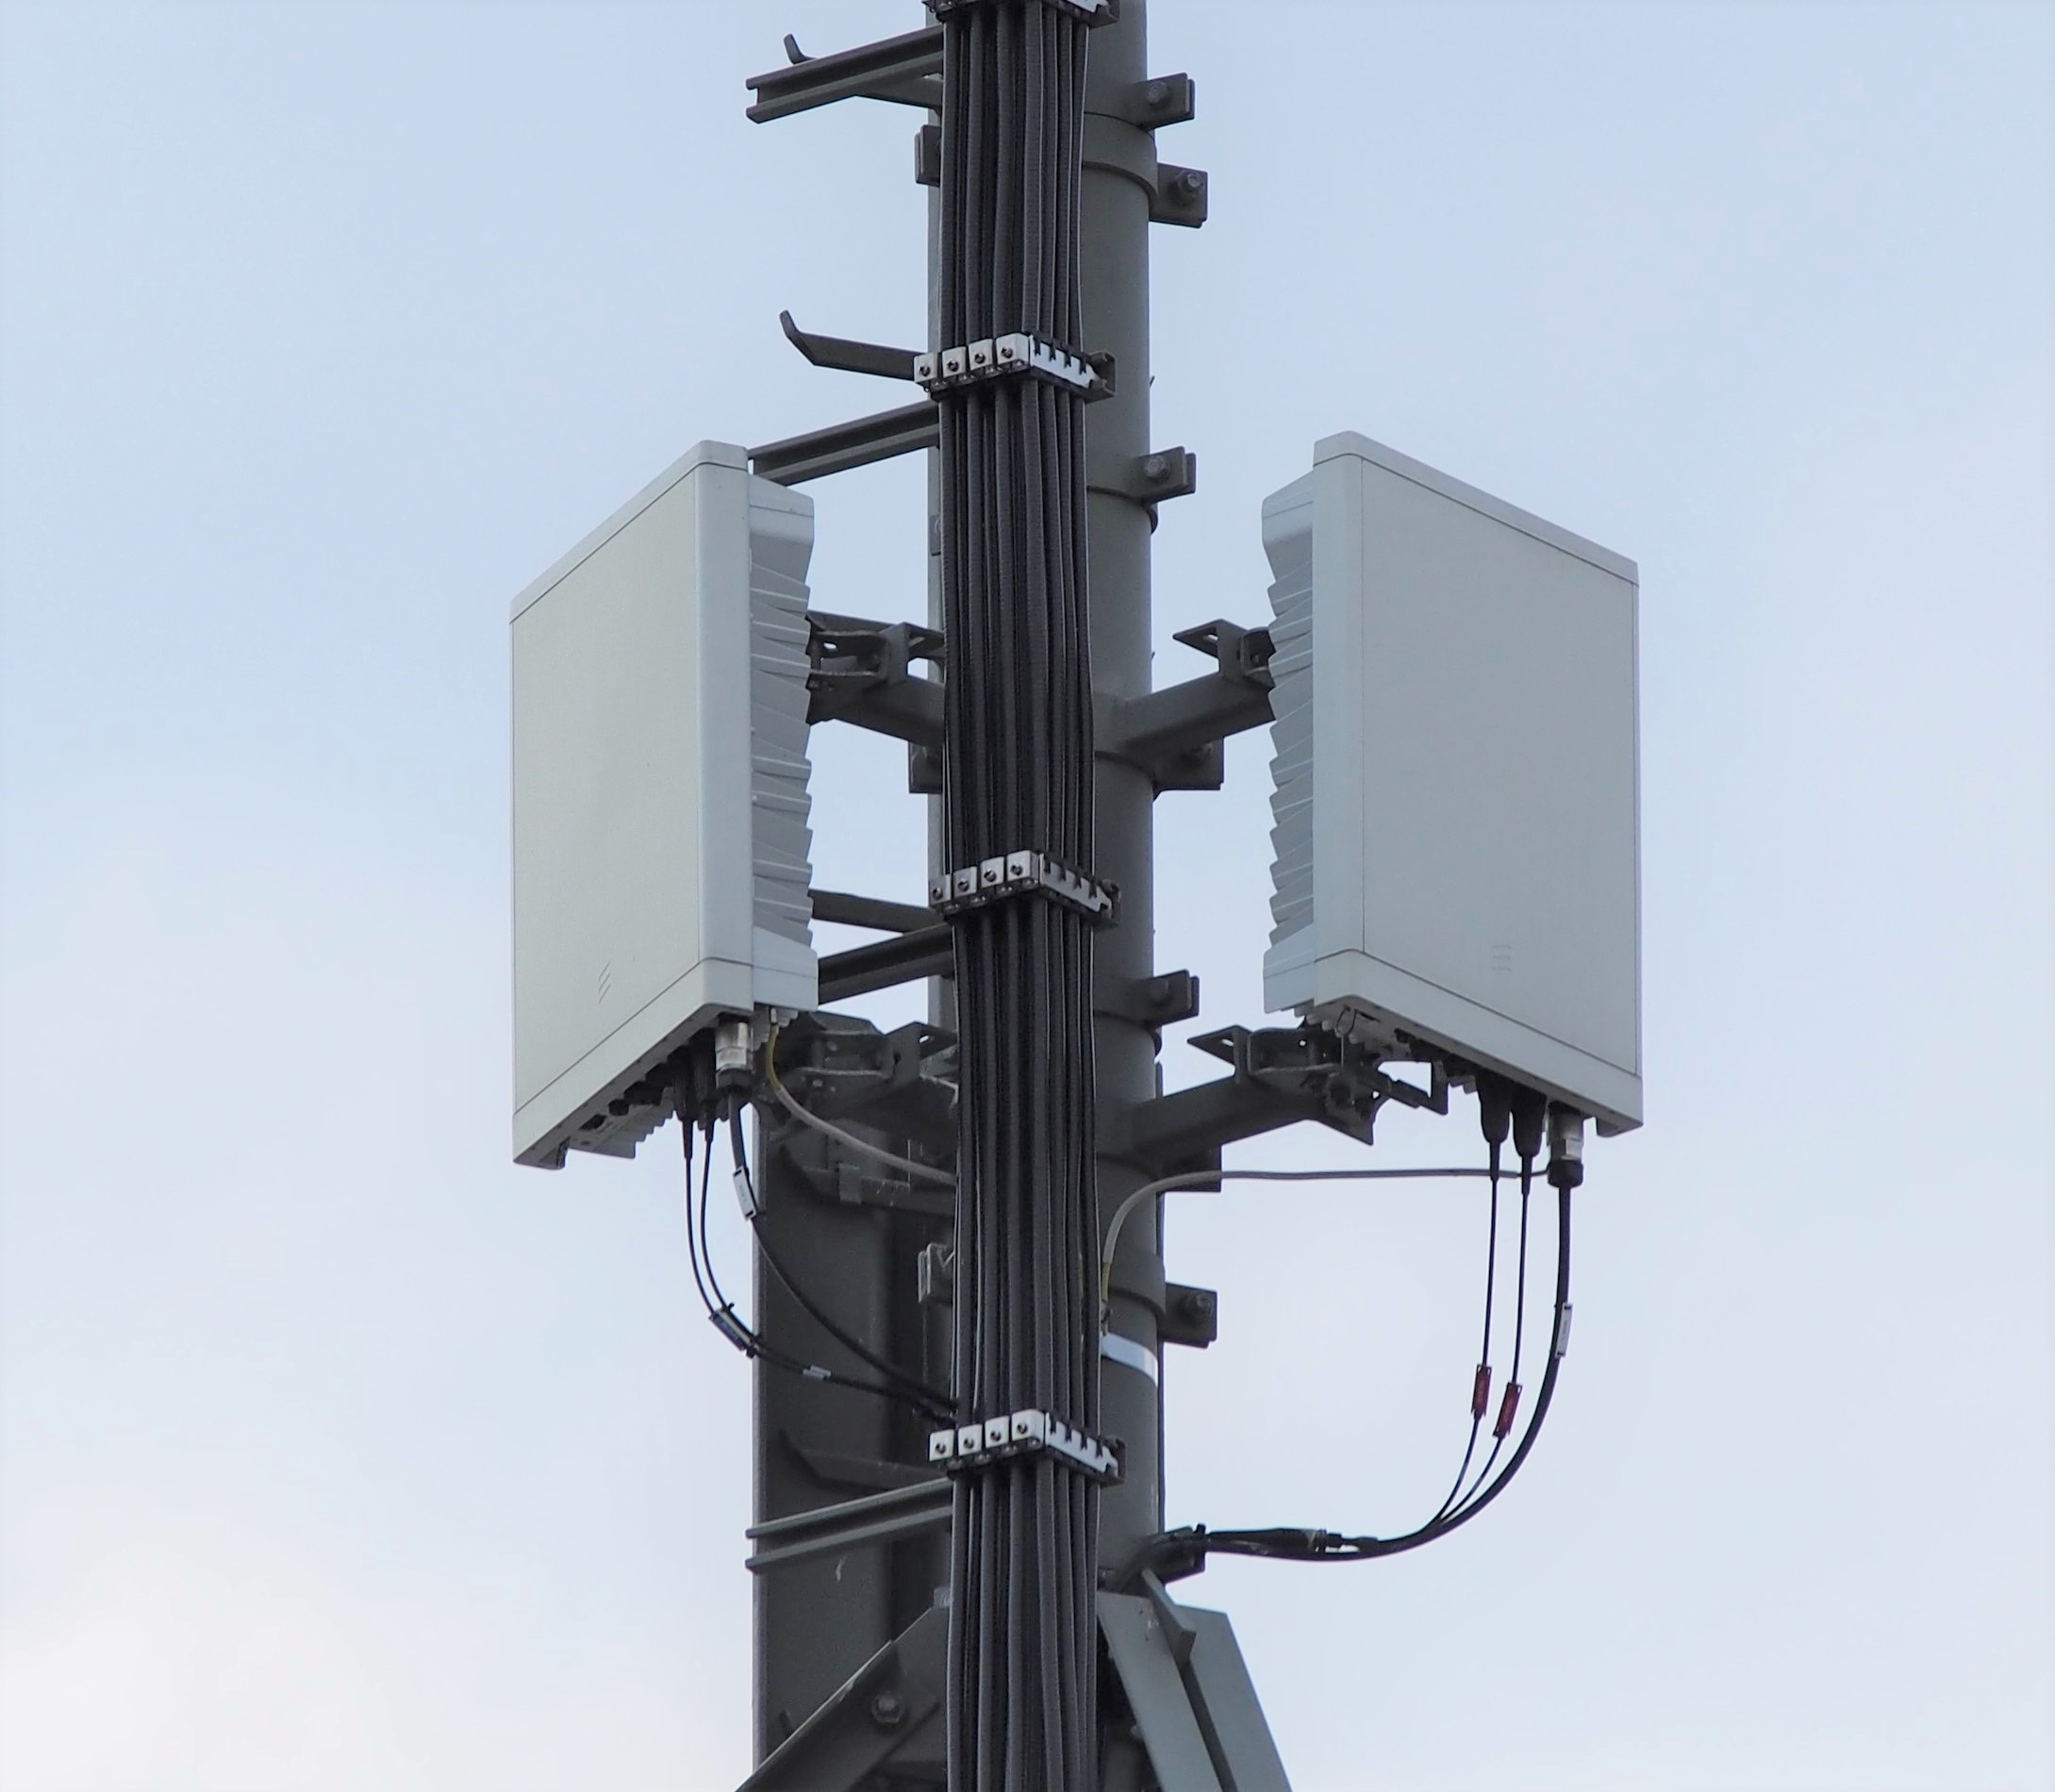
\includegraphics[width=\linewidth]{figure/xg/5g_antenna.jpg}\\
      \vspace{0.3em}
        {\footnotesize Active antenna units and dense radio sites.\par}
    \column{0.50\textwidth}
      \Large \textbf{Connectivity moves into systems.}
      \vspace{0.8em}

      \normalsize
      \begin{itemize}
        \item Enhanced mobile broadband
        \item Low-latency control and edge computing
        \item Sensing, vehicles, factories, and AI services
      \end{itemize}
     

  \end{columns}
\end{frame}

\begin{frame}{More than Technology}
  \begin{columns}[T]
    \column{0.40\textwidth}
      \centering
      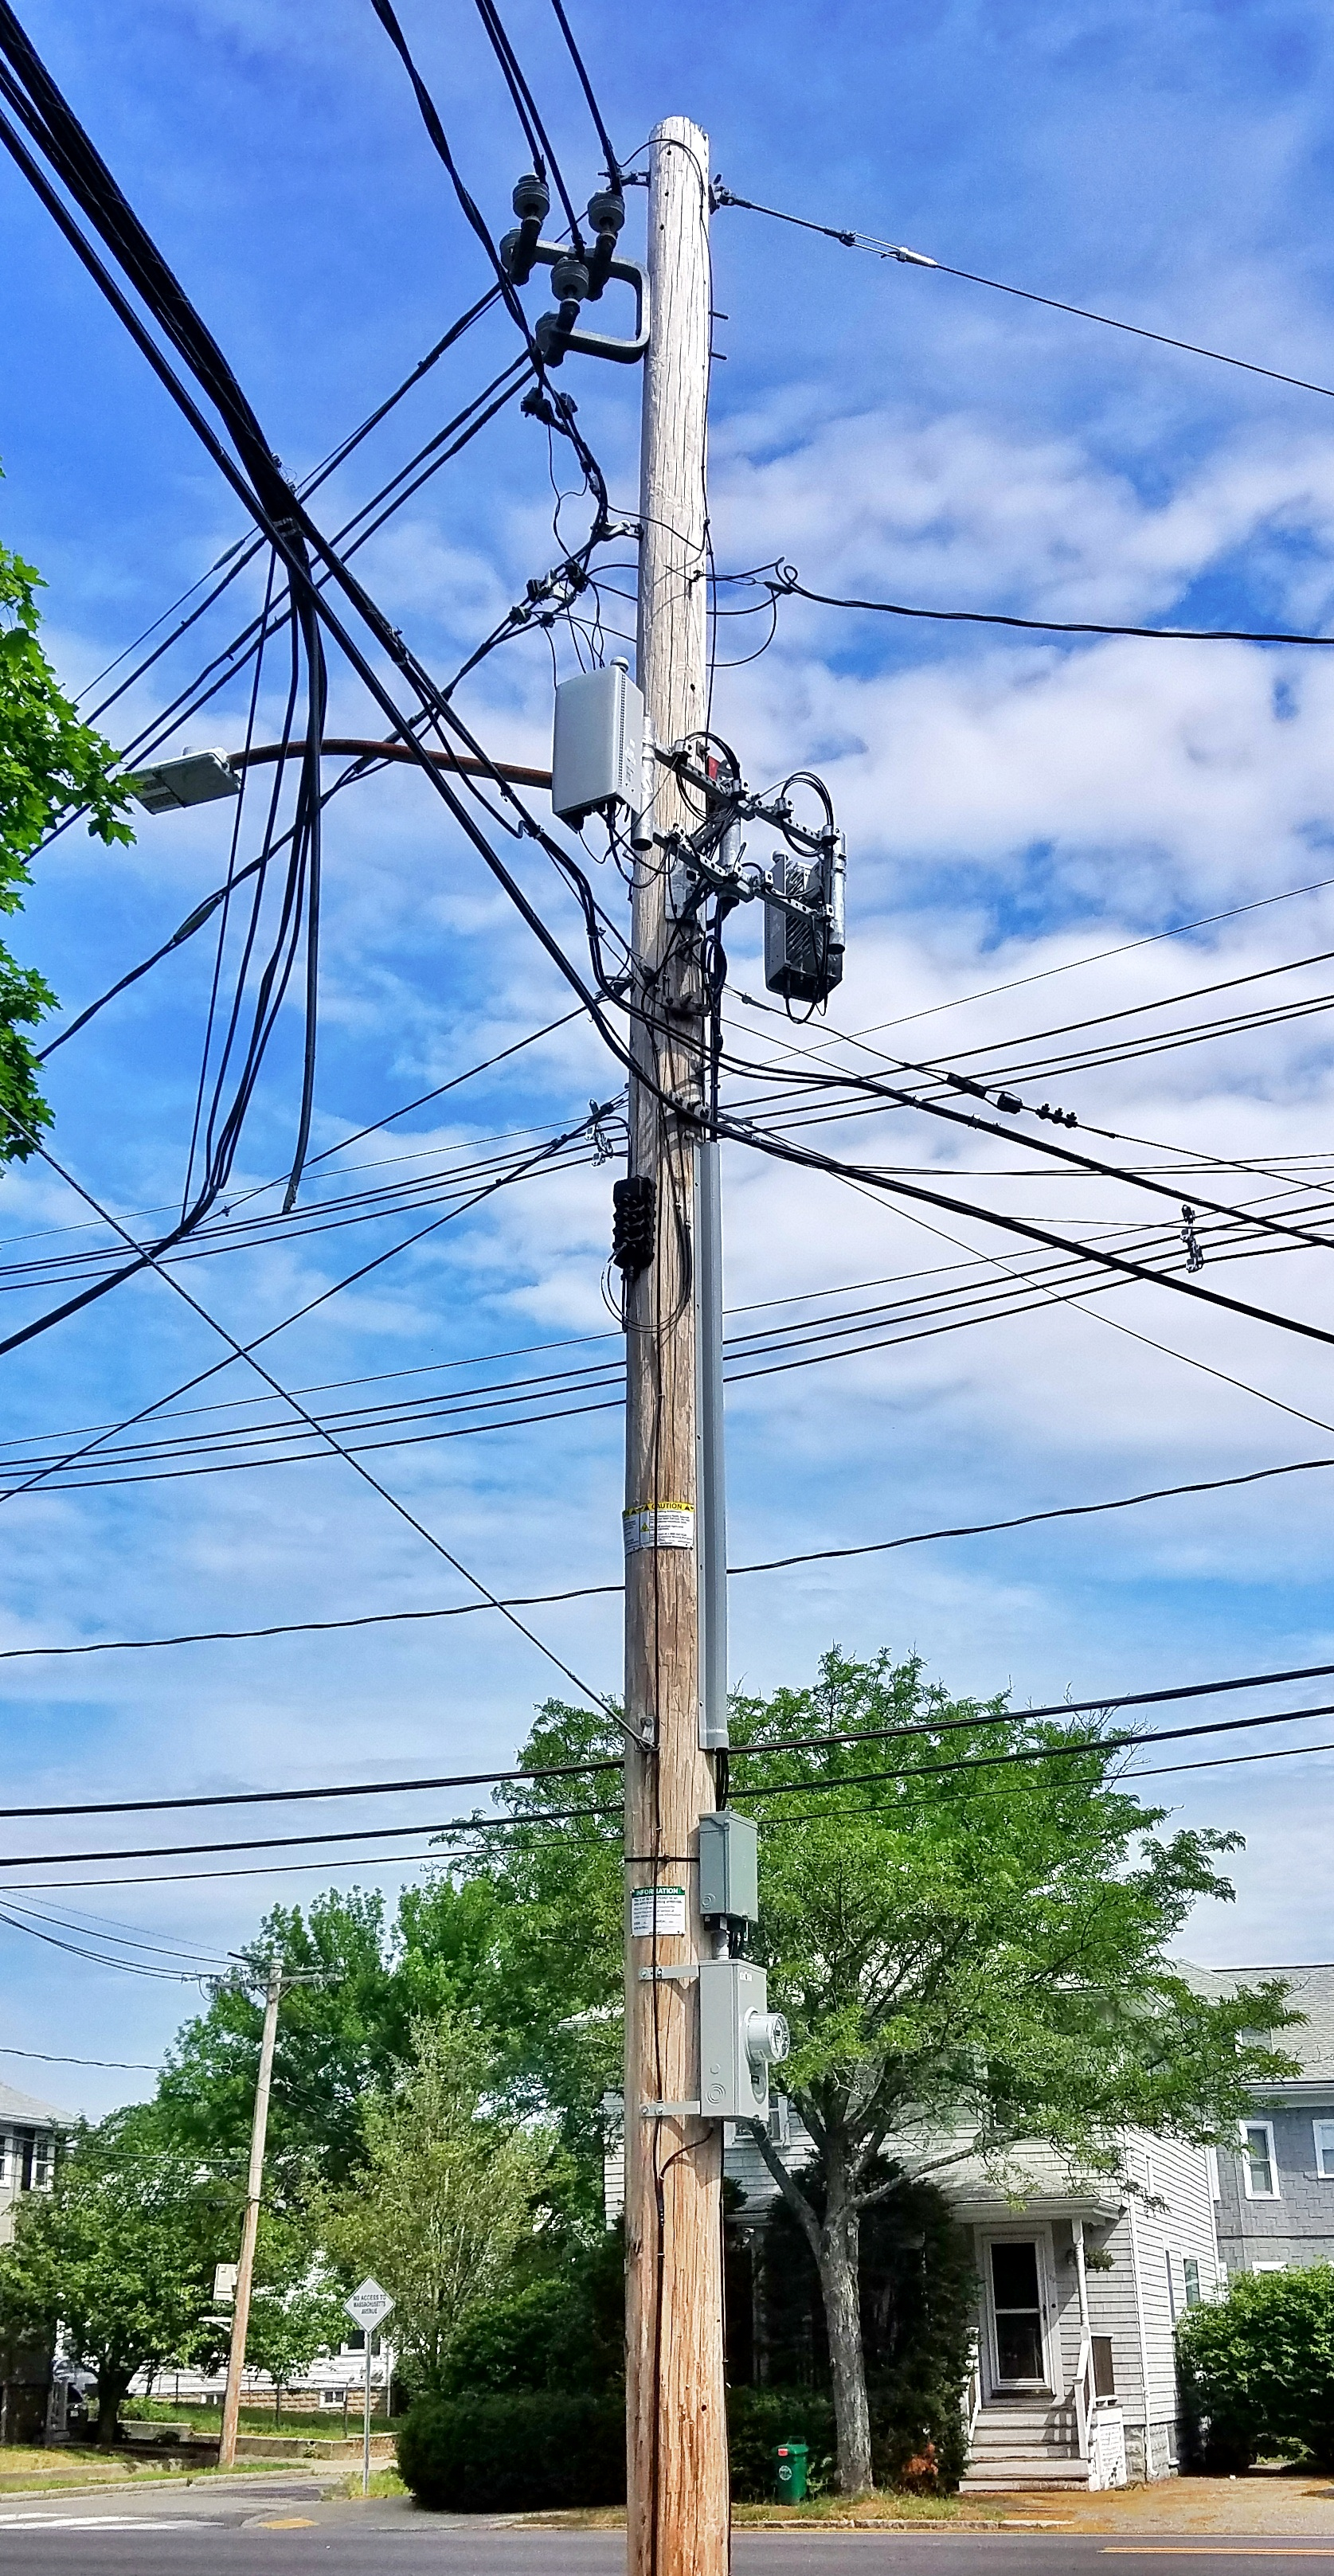
\includegraphics[height=0.7\textheight]{figure/xg/mmwave_utility_pole.jpg}\\

      \vspace{0.4em}
      {\footnotesize mmWave 5G often means dense street-level infrastructure.\par}
    \column{0.60\textwidth}
      \Large \textbf{The route matters.}
      \vspace{0.7em}

      \normalsize
      \begin{itemize}
        \item Country U had the prime mid-band spectrum tied up. Its carriers could obtain millimeter-wave spectrum more easily.
        \item Country C chose mid-band coverage first because millimeter-wave small cells cost too much at national scale.
        \item Country U fell behind in early 5G, but now returns to millimeter wave. Why? 
      \end{itemize}

  \end{columns}
\end{frame}

\begin{frame}{6G: From networks to AI systems}
  \Large
  The next ``G'' should make us ask a different question.

  \vspace{0.8em}
  \normalsize
  \begin{itemize}
    \item If every device can run or reach a large model, what should the network provide?
    \item Which tasks should stay on the device, move to nearby edge compute, or go to the cloud?
    \item What new applications appear when wireless links carry model state, sensor context, and real-time feedback?
  \end{itemize}

\end{frame}

\begin{frame}{An AI-Networking Startup: WiCi}
  \begin{columns}[T]
    \column{0.50\textwidth}
      \centering
      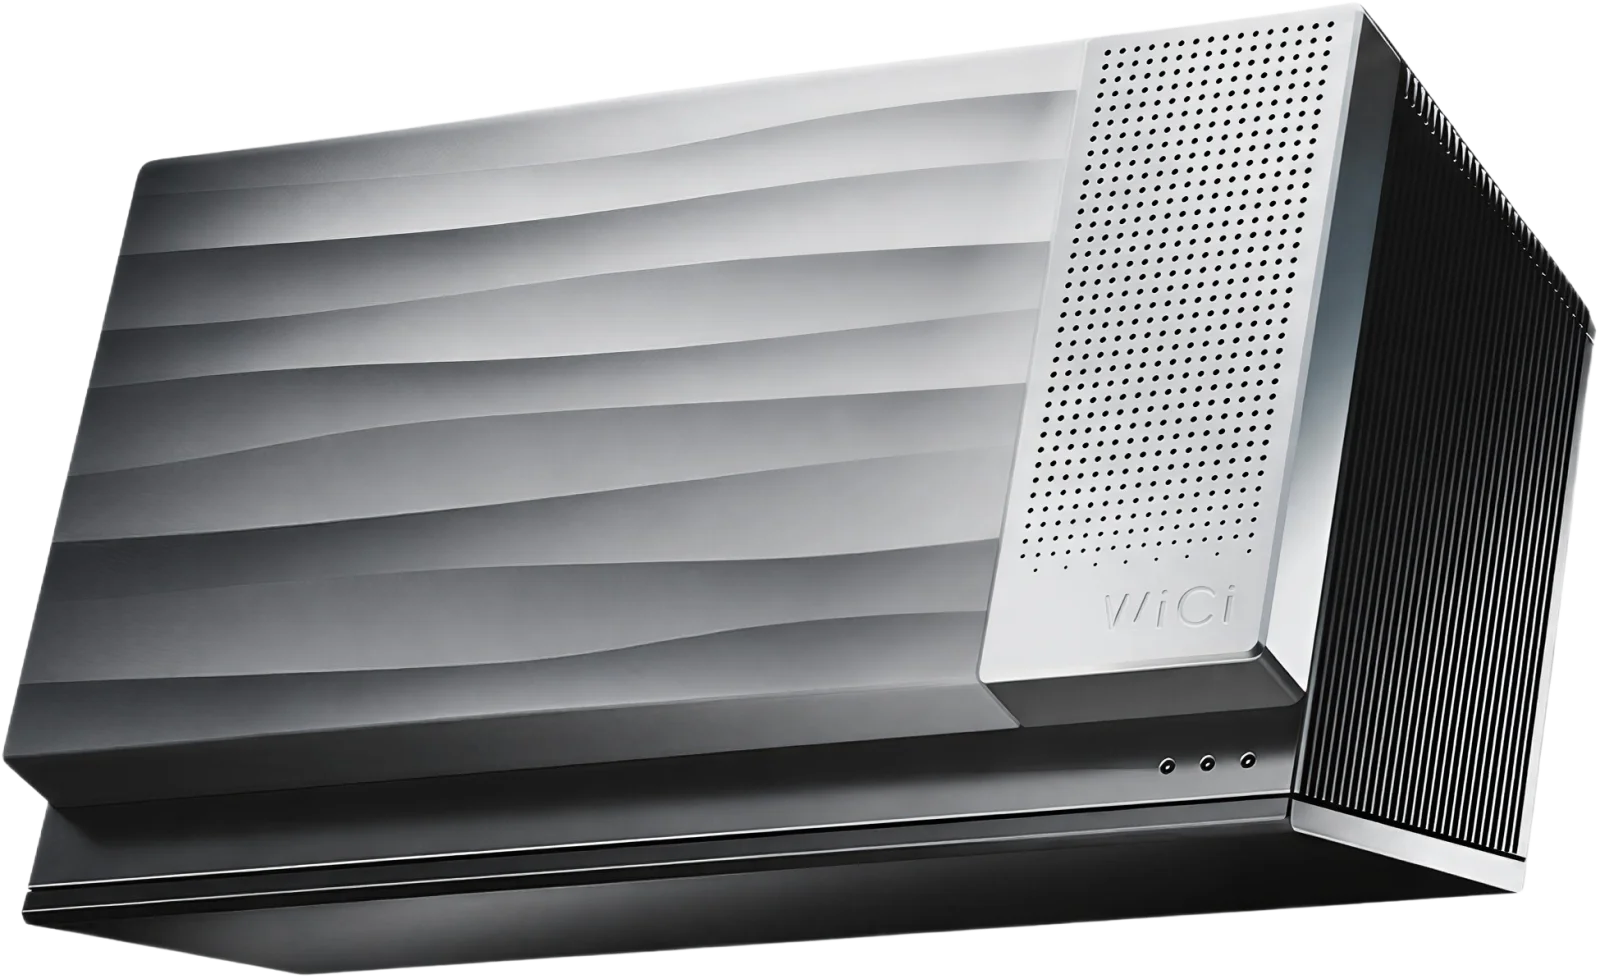
\includegraphics[width=\linewidth]{figure/xg/wici_one_product.png}\\
      \vspace{0.4em}
      \small
      \blink{https://wici.ai/wici-one}{wici.ai/wici-one}
    \column{0.50\textwidth}
      \Large \textbf{Local AI needs nearby compute.}
      \vspace{0.8em}

      \normalsize
      \begin{itemize}
        \item Phones and laptops cannot carry unlimited GPU, heat, and battery.
        \item Cloud AI adds latency, cost, privacy risk, and network dependence.
        \item WiCi One turns nearby GPU into a wireless resource.
        \item The user keeps a light device; the heavy compute stays nearby.
      \end{itemize}
  \end{columns}
\end{frame}

\begin{frame}{From 6G to XG}
  \center
  \Large
  What else could XG make possible?

\end{frame}
